\documentclass[10pt]{beamer}
\usepackage{csquotes}% Recommended
\usepackage[dvipsnames]{xcolor}

\usepackage{graphicx}
\usepackage{xcolor}
\usepackage{amsfonts}
\usepackage{amsmath}
\usepackage{amssymb}
\usepackage[skip=10pt plus1pt] {parskip}


%Information to be included in the title page:
\title{Axiomatic Probability \& Integration}
\author{UChicago Political Science Math Camp}
\institute{Ryan Gibbons \& Luke Cain}
\date{2026}

\begin{document}

\frame{\titlepage}

%=====================================================================
%  DAY 1 (Wed. 9/16)
%=====================================================================

\begin{frame}{Roadmap}

\end{frame}

\begin{frame}{}

\end{frame}

%=====================================================================
%  DAY 2 (Thurs. 9/17)
%=====================================================================

\begin{frame}{}

\end{frame}

%=====================================================================
%  SCRATCH  --  snippets to copy into frames above
%---------------------------------------------------------------------
%  Bullets:
%      \begin{itemize}
%          \item \textbf{Term:} description
%      \end{itemize}
%
%  Reveal incrementally:      \pause
%  Vertical breathing room:   \vspace{1cm}
%  Display math:              \[ f'(c) = \frac{f(b) - f(a)}{b-a} \]
%
%  Blockquote for a formal statement:
%      \begin{quote}
%          Let $f: [a,b] \rightarrow \mathbb{R}$ be continuous \ldots
%      \end{quote}
%
%  Takeaway line (house style):
%      \textit{\textcolor{red}{The intuition, stated plainly.}}
%
%  Greyed-out callback to an earlier result:
%      \[\textcolor{gray}{f'(c) = \frac{f(b)-f(a)}{b-a}}\]
%
%  Image (drop the file in this folder, no path needed):
%      \begin{center}
%          \includegraphics[width=10cm]{filename.jpg}
%      \end{center}
%=====================================================================


\begin{frame}{Probability}

Probability is the \textbf{likelihood of an event occurring} \\

\vspace{1cm}

We denote the probability of an event $A$ as a real number between 0 and 1:

\[\Pr[A] \in [0,1]\]

\end{frame}


\begin{frame}{Axioms of Probability}
    There are three basic axioms when working with probability:
    \begin{enumerate}
        \item \[\forall\; a \in A, \Pr[a] \in \mathbb{R}_+ \implies \Pr[a] \geq 0\]

        \item \[\forall A,\; \sum_{a \in A} \Pr[a] = 1\]

        \item \[a_i \cap a_{-i} = \emptyset \;\forall \;a_i, a_{-i} \iff \Pr\bigg[ \bigcup_{i=1}^k a_i\bigg] = \sum_{i=1}^k \Pr[a_i]\]
    \end{enumerate}
\end{frame}

\begin{frame}{Applying Axioms}
    Show these axioms for each of the following discrete probabilities:

    \begin{enumerate}
        \item A fair two-sided coin
        \item An unfair six-sided dice
        \item Tomorrow's temperature (in whole degrees, ok to place bounds)
    \end{enumerate}
\end{frame}

\begin{frame}{Random Variables}
    A random variable is a function $X$ such that there exists a real number for every $s \in S$:

    \[X: S \rightarrow \mathbb{R}\]

    There is then some non-deterministic probability $\Pr[X(s) = x] \in [0, 1]$ for every event $s$.
\end{frame}

\begin{frame}{PMFs}
    For a discrete random variable $X$, we can model a \textbf{probability mass function}:

    \[\text{PMF} \equiv f(x) = \Pr[X = x]\]

    This models the likelihood of any given outcome of $x \in S$. \\

    \vspace{.5cm}
    What do our probability axioms imply about PMFs?
\end{frame}

\begin{frame}{PMF examples}
    How might we construct the PMFs of the following?

    \begin{itemize}
        \item A fair, six-sided dice
        \item An unfair six-sided dice (twice as likely to land on 6)
        \item A nation's global ranking in GDP (assume $n = 200$ for simplicity
    \end{itemize}
\end{frame}

\begin{frame}{PDFs}
We use \textbf{probability density functions} (PDFs) to evaluate the ``shape'' of a continuous random variable:
\vspace{.5cm}
\begin{itemize}
    \item Uniform distribution: $f(x) = \frac{1}{b-a} \iff x \in [a,b]; 0 \text{ else}$ \pause
    \item Normal distribution: $f(x) = \frac{1}{\sigma \sqrt{2 \pi}}\exp\{\frac{-(x - \mu)^2}{2 \sigma^2}\}$ \pause
    \item Exponential distribution: $f(x) = \lambda \exp\{- \lambda x\}$
\end{itemize}

\textcolor{red}{But, moving from discrete to continuous outcomes presents a mathematical conundrum...}
\end{frame}


\begin{frame}{A Simulated Example}

Suppose you roll a \textcolor{blue}{four-sided} dice. What is the probability of rolling $1$? What is the total probability? \pause

Suppose you roll a \textcolor{blue}{six-sided} dice. What is the probability of rolling $1$? What is the total probability? \pause

Suppose you roll a \textcolor{blue}{ten-sided} dice. What is the probability of rolling $1$? What is the total probability? \pause 

Suppose you roll a \textcolor{blue}{twenty-sided} dice. What is the probability of rolling $1$? What is the total probability? \pause 

Suppose you roll a \textcolor{blue}{one-hundred-sided} dice. What is the probability of rolling $1$? What is the total probability? \pause

Suppose you roll a \textcolor{blue}{ten-thousand-sided} dice. What is the probability of rolling $1$? What is the total probability? \pause

\end{frame}


\begin{frame}{Zero-Measure Probability}
    A fundamental paradox in studying continuous random variables arises: the probability of any specific event is \textbf{measure zero}, but the random variable is non-trivial.

    This result is \emph{not} tied to the nature of the distribution, other than its continuity.

    Given this, how might we study... anything probablistic?
\end{frame}


\begin{frame}{Cumulative Probability}
Suppose we have a uniform random variable $X \sim U[0,1]$ -- that is, it takes on any value between 0 and 1 with equal probability. \pause

The probability of drawing $x = 0.5$ is measure-zero. But, the probability of drawing some number \emph{less than} $0.5$ is well-determined (and is in fact $0.5$). \pause

\textcolor{red}{While probability distributions can show relative likelihood, cumulative metrics can return \emph{exact probabilities.}}
\end{frame}



\begin{frame}{CDFs}
    We often want to represent the probability that a random variable is larger or smaller than some threshold. For this, we can model a \textbf{cumulative distribution function}:

    \[\text{CDF} \equiv F(x) = \Pr[X \leq x] = \sum_{i \leq x} \Pr[i]\]

    What do our probability axioms imply about discrete CDFs? How might we solve $\Pr[X \geq x]?$
\end{frame}

\begin{frame}{CDF examples}
    How might we construct CDFs of the following?

    \begin{itemize}
        \item A fair dice rolling at least a 3
        \item An individual being in the top $n$-th percentile of wealth
        \item The ``amount" of persuasion voters need to choose candidate $A$ in a two-race, majoritarian election
    \end{itemize}
\end{frame}


\begin{frame}{How Could We Do This?}
Our previous CDF definition lets us define cumulative probability across discrete outcomes. 

But, now we want to define cumulative probability across \emph{continuous} outcomes.

...What if we just made the ``buckets'' of discrete outcomes infinitely small?
\end{frame}

\begin{frame}
    \begin{center}
        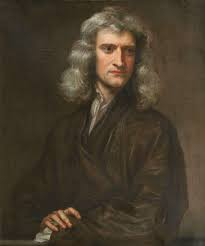
\includegraphics[width=6cm]{newton.jpeg}
    \end{center}
\end{frame}

\begin{frame}{Calculus and Infinity}

Calculus fundamentally solves the following contradictions: \\
\vspace{1cm}
\begin{itemize}

    \item Derivation solved for the rate of change of a function as $\Delta x \to 0$, such that $\frac{rise}{run} \to \infty$.
    
    \item Integration solves for the sum of an infinite number of infinitely small segments, where the size of each approaches $0$ such that $\sum_i \to 0$.

\end{itemize}

\textcolor{red}{In most cases, $\frac{rise}{run} \neq \infty$ and $\sum_i \neq 0$.}

\end{frame}

\begin{frame}{A Different Approach to Intuition}

    Say we want to measure the area bounded by some function(s), or the \textbf{area beneath the curve}:

    \begin{enumerate}
        \item If all functions are linear, we can use geometric formulas (extensions of $A = bh$) to evaluate
        \item If \underline{even one} function is non-linear\footnote{At least, non-circular, although the area of a circle is derived from calculus anyways}, then standard geometry can only approximate
    \end{enumerate}

\end{frame}

\begin{frame}{Integration From Approximation}
    We can approximate the area under a curve by splitting the area into a series of rectangles, such that $A = \sum_i bh_i$ \\

    \vspace{.5cm}

    With very large rectangles (i.e., very large $b$-values), this creates a lot of error. \textcolor{purple}{\href{https://www.desmos.com/calculator/fgqivwklhm}{But what happens}} as we add more rectangles, and shrink the size of each? \\

    \[A=\sum_i bh_i \quad \quad \implies \quad \quad b \to 0, i \to \infty\]

    \textcolor{red}{How does this reflect our derivation definition?}
\end{frame}

\begin{frame}{Notation}
    Integrate \textcolor{blue}{$f(x)$} with respect to \textcolor{red}{$x$} $\rightarrow$ What is the sum of every \textcolor{blue}{$f(x)$} over every possible \textcolor{red}{$x$}? \\

    \vspace{.5cm}

    We denote this as

    \[\int f(x) dx\]

    We call this an \textbf{indefinite integral}
\end{frame}

\begin{frame}{A New Limit Definition}
    \[\int f(x) dx = \lim_{b \to 0} \sum_i^{\frac{1}{b}}b f(x_i)\]

\end{frame}

\begin{frame}{Integration vs Derivation}
    \begin{itemize}
        \item The integral of $f(x) dx$ represents the sum of all $f$'s, such that if $f$ represents a rate of change, then $\int f(x) dx$ represents the \textbf{change that occurred...}
        \item Think: what function's derivative returns $f(x)$? That function represents $\int f(x)dx$
    \end{itemize}

To borrow again from Physics:

\[\text{\textbf{Jerk}} \Rightarrow \int{dt} = \text{\textbf{Acceleration}} \Rightarrow \int{dt} = \text{\textbf{Speed}} \Rightarrow \int dt = \text{\textbf{Position}}\]

\end{frame}

\begin{frame}{Definite vs. Indefinite Integrals}
    Often, we only want to evaluate the integral of a function over some specific domain. To integrate $f(x)$ w.r.t $x$ over the domain $[a,b]$, we write the \textbf{definite integral}

    \[\int_a^b f(x) dx\]

    \textcolor{red}{An indefinite integral often produces a function. A definite integral almost always returns a number (or function independent of $x$).}
\end{frame}

\begin{frame}{FTOC}

\[\int_a^b f'(x)dx = f(b) - f(a)\]

This yields two truths:

\begin{enumerate}
    \item The integral is the inverse of the derivative (the integral of a function's derivative is just the function)
    \item For some defined domain $[a,b]$, the value of the integral over that domain is $\int f(b)dx - \int f(a)dx$
\end{enumerate}

\end{frame}

\begin{frame}{FTOC and Indefinite Integrals}
    Let's reiterate an important point here: \\

    \vspace{.5cm}

    If we denote the indefinite integral $\int f(x)dx = F$, then $\int_a^b f(x)dx = F(b) - F(a)$ \\

    \vspace{.5cm}

    Then, to solve $\int_a^b f(x)dx$, we evaluate:

    \[\int f(x) dx = F(x) \quad \implies \quad \int_a^b f(x)dx = F(x) \bigg|_{x=a}^{x=b}\]
\end{frame}

\begin{frame}
    \thispagestyle{empty}
    \vspace{1cm}
    \begin{center}
        \begin{Huge}
            How Do We Actually Do This?
        \end{Huge}
    \end{center}
\end{frame}


\begin{frame}{The Good Stuff}
    We can use a series of rules to integrate a function in its general form \textit{\underline{for any value of $x$}}:

    \[f(x) \implies \text{[RULE]} \implies \int f(x) dx\]

    Note that now, our indefinite integral is itself another function of $x$.
\end{frame}

\begin{frame}{The Sum Rule}
    For all integrals:

    \[\int \Big[f(x) + g(x)\Big] dx  = \int f(x) dx + \int g(x) dx\]

    For definite integrals such that $a \leq b \leq c$:

    \[\int_a^c f(x) dx = \int_a^b f(x) dx + \int_b^c f(x)dx\]
\end{frame}

\begin{frame}{The Power Rule, Backwards}
    Recall the derivative power rule:

    \[\frac{d}{dx} x^k = k \cdot x^{k-1}\]

    Then, if $\int f'(x) dx = f(x)$, what function would, when derived, produce ours? \pause

    \[\int x^k dx = \frac{x^{k+1}}{k+1}\]

    plus one little thing...
\end{frame}

\begin{frame}{Remember Our Constants?}
    \begin{enumerate}
        \item We know that the derivative of a constant is $0$, such that $\frac{d}{dx} c = 0 \; \forall \; c \in \mathbb{R}$
        \item If integration ``reverts" a derivative, then it must account for any constant terms zero-d out in derivation
        \item We resolve this as follows:

        \[\int x^k dx = \frac{x^{k+1}}{k+1} + c\]

         \textit{even though we don't know what $c$ actually is.}
    \end{enumerate}
\end{frame}

\begin{frame}{A Power Rule Corollary (Reversed)}
    \begin{enumerate}
        \item We know that $\int x^k dx = \frac{1}{k+1} x^{k + 1}$ (\textbf{Power Rule}) and that $\int [f(x) + g(x)] dx = \int f(x) dx + \int g(x) dx$ (\textbf{Sum Rule})
        \item We also know that for a constant $\ell$, $\ell \cdot n = \sum_1^\ell n$, or $n$ added $\ell$ times. 
        \item Then, the integral is the sum of $x^k$ added up $\ell$ times:
        \[\int \bigg[ \ell \cdot x^k\bigg] dx = \sum_1^\ell \int x^k dx\]
        \item We know that $\sum_1^n x = nx$, so
        \[\sum_1^\ell \int x^k dx = \ell \cdot \int x^k dx \quad \implies \quad \int \bigg[ \ell \cdot x^k \bigg] dx = \ell \cdot \frac{1}{k+1} \cdot x^{k + 1}\]
    \end{enumerate}

    $\implies$  \textbf{Coefficients}: The coefficient of a term is kept as a coefficient of that term's integral (i.e., multiply $\frac{1}{k+1}$ by the coefficient as well)
\end{frame}

\begin{frame}{Quick Note on Constants}
    Recall that a constant $m$ can be represented as $m \cdot x^0$. Then,

    \[\int mdx = \int m \cdot x^0 dx\]
    \[\implies m \cdot \int x^0 dx\]
    \[\implies m \cdot \frac{x^{0+1}}{0+1} + c= m \cdot \frac{x^1}{1} + c\]
    
    \[\therefore \int m dx = mx + c\]
\end{frame}

\begin{frame}{Some Examples}
    Let's try some simple examples:

    \[\int x^2 + 2x^3 dx\] \pause

    \[\int 2x^3 + \frac{1}{2} x^4  dx \] \pause

    \[\int 3 + \sqrt[3]{x} dx\] \pause

    \[\int x^{-3} + x^{-2} + x^{-1} dx\] 
\end{frame}

\begin{frame}{Closing Some Subtle Foreshadowing}
    The power rule doesn't work for $f(x) = x^{-1} = \frac{1}{x}$, as it solves:

    \[\int x^{-1} dx = \frac{1}{-1+1} x^{-1 + 1} = - \frac{x^0}{0}\]

    Thankfully, our natural logarithm solves this for us:

    \[\int \frac{1}{x} dx = \ln(x) + c\]
\end{frame}

\begin{frame}{Integrating Exponentials}
    We have a specific rule for integrating exponentials and logarithms:

    \[\int a^x dx  = \frac{a^x}{\ln a} + c\]

    \[\int \log_b x dx = \frac{x}{\ln b} (\ln b - 1) + c\]
\end{frame}

\begin{frame}{Definite Integration}
    So far, we've expressed $F(x)$ for every $f(x)$, both as functions of $x$, as \textit{indefinite integrals}. When we add bounds of integration, we simply use FTOC:

    \[\int_a^b f(x)dx = F(b) - F(a)\]

    \[\int_2^4 x^3 dx \quad = \quad \int x^3 dx \bigg|_2^4 \]

    \[\implies \frac{x^4}{4} + c \;\bigg|_2^4\]

    But, we don't know $c$...
\end{frame}

\begin{frame}{$c$ you later}
    There's a handy trick with definite integrals:

    \[\int f(x) dx = F(x) + c\]
    \[\implies \int_a^b f(x) dx = F(b) + c - \Big( F(a) + c\Big)\]
    \[\implies \int_a^b f(x) dx = F(b) - F(a)\]

    For definite integrals, we subtract $c-c$ and can therefore exclude it. So,

    \[\frac{x^4}{4} + c \; \bigg|_2^4 \quad = \quad \frac{4^4}{4} - \frac{2^4}{4} \quad = 16\]
\end{frame}

\begin{frame}{More Examples}
    \[\int_0^2 x^3 + 2x^3 dx\] \pause

    \[\int_2^6 \frac{1}{2} x^2 + 4 dx\] \pause 

    \[\int_0^b \sqrt{x} + \sqrt{2} dx\] \pause

    \[\int_{a}^{2} \frac{1}{x^2} dx\] \pause
\end{frame}

\begin{frame}{A Turn For The Worst}
    Two of our fundamental derivative rules -- the \textbf{chain rule} and the \textbf{product rule} -- are a bit more complicated to invert:

    \[\frac{d}{dx}f(u) = f'(u) \cdot u'\]

    \[\implies F(u) = \int f(u) \cdot u du...\]

    There's not a clear solution here
\end{frame}

\begin{frame}{U-Substitution}
    The inverse of the Chain Rule is called \textbf{integration by substitution}, or \textbf{``u-sub"}, and works as follows:

    \begin{enumerate}
        \item Express the integral in the form
        \[\int f\Big(g(x)\Big) g'(x) dx\]
        \item Assign $g(x) = u$ such that the integral can be rewritten:
        \[ \int f(u) du\]
        \item Evaluate the integral:
        \[\int f(u) du = F(u)\]
        \item Substitute back $u = g(x)$:
        \[\int f\Big(g(x)\Big) g'(x) dx = F\Big(g(x)\Big)\]
    \end{enumerate}
\end{frame}

\begin{frame}{Integration By Parts}
    \textbf{Integration by parts} inverts the product rule. We will not cover it in math camp, but you should be aware of the concept and ready to learn its process.
\end{frame}

\begin{frame}{Improper Integrals}
    For definite integrals which do not converge to $f(x) = a$, or for any asymmetric integrals whereby $f(x) = \pm \infty$ for $x \in \mathbb{R}$, we call that integral \textbf{improper.} \\

    \vspace{.5cm}

    This can either result in a finite value, such as $\int_{-\infty}^{\infty} \frac{1}{1+x^2}dx$, or an undefined value, such as $\int_{-\infty}^{\infty} \frac{1}{x} dx$
\end{frame}

\begin{frame}{Gabriel's Horn}
    Imagine a horn formed by the function $f = \frac{1}{x}$ for the domain $x \in [1, \infty)$

    What is its volume? What is its surface area?
\end{frame}

\begin{frame}{Horn Volume}
    We know that $V = a \cdot h$; in this case we can set $h = \infty$ and $a = \pi r(x)^2 =\frac{\pi}{x^2}$. The volume is then the sum of this area over every possible height:

    \[V = \int_1^\infty \frac{\pi}{x^2} dx = - \frac{\pi}{x} \bigg|_1^{\infty} \]

    \[V = \pi\]

    The volume of the horn is finite.
\end{frame}

\begin{frame}{Horn Surface Area}
    We know that surface area can be calculated as $s = c \cdot h$. In this case, we set $h = \infty$ and $c = \pi 2r = \frac{2\pi}{x}$. The surface area is then the sum of this circumference over every possible diameter:

    \[s = \int_1^{\infty} \frac{2 \pi}{x} dx = 2\pi \cdot \ln(x) \bigg|_1^{\infty}\]

    \[s = \infty\]

The horn has finite volume but infinite surface area. \textit{You could fill the inside with paint, but never fully paint the outside.}
\end{frame}


\begin{frame}{Expectation}

You've already seen the expectation operator for discrete random variables:

\begin{align*}
    \mathbb{E}[X] &= \sum_{x \in X}x \cdot \Pr[X = x]
\end{align*}

How might we apply this to continuous random variables?
\pause

\textcolor{red}{Send $\#\{X\} \to \infty$ and $\Pr[X = x] \to \frac{1}{\infty}$.} 

\end{frame}

\begin{frame}{Expectation With Infinite Outcomes}
    If we're just taking an infinite sum of infinitely small pieces, we're taking an integral.

    This yields our continuous expectation function:

    \begin{align*}
        \mathbb{E}[X] &= \int_{x \in X} x f(X) dx
    \end{align*}

    where $f(x)$ is the PDF.
\end{frame}

\begin{frame}{Example}

    Suppose we have an exponential distribution where $f: \mathbb{R}_+ \to \mathbb{R}_+$:
    \begin{align*}
        f(x) &= \lambda \exp\{- \lambda x\}
    \end{align*}

    \pause

    We can integrate accordingly:
    \begin{align*}
        \mathbb{E}[f(x)] &= \int x f(x) dx \\
        &= \int_{0}^\infty x \lambda e^{- \lambda x} dx \\
        &= \frac{1}{\lambda}
    \end{align*}

\end{frame}

\begin{frame}{Expected Utility}
Often, we have two functions (i.e., a PDF and a utility function), and we want to know the expectation of their product.

We can use a relatively simple integral:

\begin{align*}
    \mathbb{E}[u(X)] &= \int_\mathbb{R} u(x) f(x) dx
\end{align*}

\end{frame}

\begin{frame}{An Example: Risk vs. Reward}

Suppose we play some lottery where (1) returns are marginally increasing and (2) higher rewards are less likely than lower rewards:

\begin{align*}
    f(x) &= \lambda \exp \{- \lambda x\} \\
    u(x) &= \lambda x a
\end{align*}

 for $a > 1$. What is the expected value of this lottery?

\end{frame}

\begin{frame}{Answer}
\begin{align*}
    \mathbb{E}[u(X)] &= \int_\mathbb{R} f(x) u(x) dx \\
    &= \int_0^\infty \lambda \exp \{- \lambda x\} x^a dx \\
    &= a
\end{align*}
\end{frame}

\begin{frame}{Let us Optimize}

If you were playing the above lottery, how would you manipulate $\lambda,a$ to maximize your expected utility?

\end{frame}

\end{document}
